\documentclass[expanded]{lkx_pset}

\title{CS181 Problem Set 4}
\author{Lev Kruglyak}
\due{March 29, 2024}

\usepackage{pgfplots}
\pgfplotsset{compat=1.14}
\usepackage[outputdir=build]{minted}
\usepackage{graphicx}

\usepackage{amsmath}
\usepackage{amssymb}
\usepackage{graphicx}
\usepackage{tikz}
\usetikzlibrary{patterns}
\usepackage{subfig}
\usepackage{comment}

\newcommand{\boldA}{\mathbf{A}}
\newcommand{\boldB}{\mathbf{B}}
\newcommand{\boldC}{\mathbf{C}}
\newcommand{\boldD}{\mathbf{D}}
\newcommand{\boldE}{\mathbf{E}}
\newcommand{\boldF}{\mathbf{F}}
\newcommand{\boldG}{\mathbf{G}}
\newcommand{\boldH}{\mathbf{H}}
\newcommand{\boldI}{\mathbf{I}}
\newcommand{\boldJ}{\mathbf{J}}
\newcommand{\boldK}{\mathbf{K}}
\newcommand{\boldL}{\mathbf{L}}
\newcommand{\boldM}{\mathbf{M}}
\newcommand{\boldN}{\mathbf{N}}
\newcommand{\boldO}{\mathbf{O}}
\newcommand{\boldP}{\mathbf{P}}
\newcommand{\boldQ}{\mathbf{Q}}
\newcommand{\boldR}{\mathbf{R}}
\newcommand{\boldS}{\mathbf{S}}
\newcommand{\boldT}{\mathbf{T}}
\newcommand{\boldU}{\mathbf{U}}
\newcommand{\boldV}{\mathbf{V}}
\newcommand{\boldW}{\mathbf{W}}
\newcommand{\boldX}{\mathbf{X}}
\newcommand{\boldY}{\mathbf{Y}}
\newcommand{\boldZ}{\mathbf{Z}}
\newcommand{\bolda}{\mathbf{a}}
\newcommand{\boldb}{\mathbf{b}}
\newcommand{\boldc}{\mathbf{c}}
\newcommand{\boldd}{\mathbf{d}}
\newcommand{\bolde}{\mathbf{e}}
\newcommand{\boldf}{\mathbf{f}}
\newcommand{\boldg}{\mathbf{g}}
\newcommand{\boldh}{\mathbf{h}}
\newcommand{\boldi}{\mathbf{i}}
\newcommand{\boldj}{\mathbf{j}}
\newcommand{\boldk}{\mathbf{k}}
\newcommand{\boldl}{\mathbf{l}}
\newcommand{\boldm}{\mathbf{m}}
\newcommand{\boldn}{\mathbf{n}}
\newcommand{\boldo}{\mathbf{o}}
\newcommand{\boldp}{\mathbf{p}}
\newcommand{\boldq}{\mathbf{q}}
\newcommand{\boldr}{\mathbf{r}}
\newcommand{\bolds}{\mathbf{s}}
\newcommand{\boldt}{\mathbf{t}}
\newcommand{\boldu}{\mathbf{u}}
\newcommand{\boldv}{\mathbf{v}}
\newcommand{\boldw}{\mathbf{w}}
\newcommand{\boldx}{\mathbf{x}}
\newcommand{\boldy}{\mathbf{y}}
\newcommand{\boldz}{\mathbf{z}}

\newcommand{\mcA}{\mathcal{A}}
\newcommand{\mcB}{\mathcal{B}}
\newcommand{\mcC}{\mathcal{C}}
\newcommand{\mcD}{\mathcal{D}}
\newcommand{\mcE}{\mathcal{E}}
\newcommand{\mcF}{\mathcal{F}}
\newcommand{\mcG}{\mathcal{G}}
\newcommand{\mcH}{\mathcal{H}}
\newcommand{\mcI}{\mathcal{I}}
\newcommand{\mcJ}{\mathcal{J}}
\newcommand{\mcK}{\mathcal{K}}
\newcommand{\mcL}{\mathcal{L}}
\newcommand{\mcM}{\mathcal{M}}
\newcommand{\mcN}{\mathcal{N}}
\newcommand{\mcO}{\mathcal{O}}
\newcommand{\mcP}{\mathcal{P}}
\newcommand{\mcQ}{\mathcal{Q}}
\newcommand{\mcR}{\mathcal{R}}
\newcommand{\mcS}{\mathcal{S}}
\newcommand{\mcT}{\mathcal{T}}
\newcommand{\mcU}{\mathcal{U}}
\newcommand{\mcV}{\mathcal{V}}
\newcommand{\mcW}{\mathcal{W}}
\newcommand{\mcX}{\mathcal{X}}
\newcommand{\mcY}{\mathcal{Y}}
\newcommand{\mcZ}{\mathcal{Z}}

\newcommand{\reals}{\ensuremath{\mathbb{R}}}
\newcommand{\integers}{\ensuremath{\mathbb{Z}}}
\newcommand{\rationals}{\ensuremath{\mathbb{Q}}}
\newcommand{\naturals}{\ensuremath{\mathbb{N}}}
\newcommand{\trans}{\ensuremath{\mathsf{T}}}
\newcommand{\ident}{\mathbf{I}}
\newcommand{\bzero}{\mathbf{0}}

\newcommand{\balpha}{\mathbf{\alpha}}
\newcommand{\bbeta}{\mathbf{\beta}}
\newcommand{\bdelta}{\mathbf{\delta}}
\newcommand{\boldeta}{\mathbf{\eta}}
\newcommand{\bkappa}{\mathbf{\kappa}}
\newcommand{\bgamma}{\mathbf{\gamma}}
\newcommand{\bmu}{\boldsymbol{\mu}}
\newcommand{\bphi}{\mathbf{\phi}}
\newcommand{\bpi}{\boldsymbol{\pi}}
\newcommand{\bpsi}{\mathbf{\psi}}
\newcommand{\bsigma}{\mathbf{\sigma}}
\newcommand{\btheta}{\mathbf{\theta}}
\newcommand{\bxi}{\mathbf{\xi}}
\newcommand{\bGamma}{\mathbf{\Gamma}}
\newcommand{\bLambda}{\mathbf{\Lambda}}
\newcommand{\bOmega}{\mathbf{\Omega}}
\newcommand{\bPhi}{\mathbf{\Phi}}
\newcommand{\bPi}{\mathbf{\Pi}}
\newcommand{\bPsi}{\mathbf{\Psi}}
\newcommand{\bSigma}{\mathbf{\Sigma}}
\newcommand{\bTheta}{\mathbf{\Theta}}
\newcommand{\bUpsilon}{\mathbf{\Upsilon}}
\newcommand{\bXi}{\mathbf{\Xi}}
\newcommand{\bepsilon}{\mathbf{\epsilon}}

\def\argmin{\operatornamewithlimits{arg\,min}}

\newcommand{\given}{\,|\,}
\newcommand{\distNorm}{\mathcal{N}}

\newcommand{\mueps}{\mu_{\epsilon}}
\newcommand{\sigeps}{\sigma_{\epsilon}}
\newcommand{\mugam}{\mu_{\gamma}}
\newcommand{\siggam}{\sigma_{\gamma}}
\newcommand{\muzp}{\mu_{p}}
\newcommand{\sigzp}{\sigma_{p}}
\newcommand{\gauss}[3]{\frac{1}{2\pi#3}e^{-\frac{(#1-#2)^2}{2#3}}}


\collaborator{Artemas Radik}
\collaborator{AJ LaMotta}
\collaborator{Leonardo Kaplan}
\collaborator{GPT-4 (for help with debugging code)}

\begin{document}
\maketitle

\begin{problem}{1}[Fitting an SVM by hand]
Consider a dataset with the following 7 data points each with $x \in \reals$ and $y \in \{ -1, +1 \}$ : \[\{(x_i, y_i)\}_{i = 1}^7 =\{(-3 , +1) , (-2 , +1 ) , (-1,  -1 ), (0, +1), ( 1 , -1 ), ( 2 , +1 ) , (3 , +1 )\}\] Consider
mapping these points to $2$ dimensions using the feature vector $\bphi(x) =  (x, -\frac{8}{3}x^2 + \frac{2}{3}x^4 )$. The hard margin classifier training problem is:
\begin{align*}
	                        & \min_{\mathbf{w}, w_0} \frac{1}{2}\|\mathbf{w}\|_2^2 \label{eq:dcp}               \\
	\quad \text{s.t.} \quad & y_i(\mathbf{w}^\top \bphi(x_i) + w_0) \geq 1,~\forall i \in \{1,\ldots, n\}\notag
\end{align*}
\end{problem}

\begin{parts}
	\begin{part}{1}
		Plot the transformed training data in $\reals^2$ and draw the optimal decision boundary of the max margin classifier. You can determine this by inspection (i.e. by hand, without actually doing any calculations).
	\end{part}

	Here is a plot of the transformed training data with decision boundary at $\varphi_2(x) = -1$:
	\begin{center}
		\begin{tikzpicture}
			\begin{axis}[title={Transformed Data Points and Approximate Decision Boundary}, ylabel={$-\frac{8}{3}x^2+\frac{2}{3}x^4$}, xlabel={$x$}, legend pos=north west, grid=both, xmin=-4, xmax=4, ymin=-10, ymax=35]

				\addplot[only marks, mark=*, mark options={fill=blue}] coordinates {
						(-3, 30) (-2, 0) (0, 0) (2, 0) (3, 30)
					};

				\addplot[only marks, mark=*, mark options={fill=red}] coordinates {
						(-1, -2) (1, -2)
					};

				\legend{+1,-1}

				\addplot[domain=-4:4, samples=2, dashed] {-1+x*0};
			\end{axis}
		\end{tikzpicture}
	\end{center}

	\begin{part}{2} What is the value of the margin achieved by the optimal
		decision boundary found in Part 1?
	\end{part}

	The optimal decision boundary has margin $1$ since this is the closest distance from the decision boundary to the points $(-1, 2), (0,0), (1,-2)$.

	\begin{part}{3} Identify a unit vector that is orthogonal to the decision boundary.
	\end{part}

	Since the decision boundary is a horizontal line, a unit vector orthogonal to the decision boundary is the vertical vector $(0,1)^\intercal$ or $(0,-1)^\intercal$.

	\begin{part}{4} Considering the discriminant $h(\bphi(x);\boldw,w_0)=\boldw^\top\bphi(x) +w_0$,
		give an expression for {\em all possible} $(\boldw,w_0)$ that define
		the decision boundary. Justify your answer.
	\end{part}

	Since $(0,1)^\intercal$ is a vector orthogonal to the decision boundary, the weight $\boldw$ must be of the form $(0,c)^\intercal$ for some $c\in \R^\times$. This means that $w_0=c$. Thus,
	\[
		(\boldw, w_0) \in \{ ((0,c)^\intercal, c) : c\in \R^\times \}.
	\]

	\begin{part}{5} Consider now the training problem for this dataset. Using your answers so far,
		what particular solution to $\boldw$ will be optimal for the
		optimization problem?
	\end{part}

	If we assume that $\boldw=(0,c)^\intercal$ and $w_0=c$, the constraint just becomes $c\geq 1$, and we want to minimize $\|w\|_2^2 = c^2$ so $c=1$. Thus the optimal solution is $\boldw(0,1)^\intercal$.

	\begin{part}{6} What is the corresponding optimal value of $w_0$ for the $\boldw$ found in Part 5 (use your result from Part 4 as guidance)? Substitute in these optimal values and write out the discriminant function
		$h(\bphi(x);\boldw,w_0)$ in terms of the variable $x$ .
	\end{part}

	Since the optimal $w_0=1$, the discriminant is now
	\[
		h(\phi(x); \boldw, w_0) = 1-\frac{8}{3}x^2 + \frac{2}{3}x^4.
	\]

	\begin{part}{7} Which points could possibly be support vectors of the classifier?  Confirm that
		your solution in Part 6 makes the constraints above tight---that is,
		met with equality---for these candidate points.
	\end{part}

	We can find five support vectors, i.e. $(2,1), (-2,-1),$ and $(0,1)$. We can verify each of these
	\[
		\begin{aligned}
			1 & = 1-\frac{8}{3}(\pm 2)^2 +\frac{2}{3}(\pm 2)^4,                  \\
			1 & = -1\left(1-\frac{8}{3}(\pm 1)^2  + \frac{2}{3}(\pm 1)^4\right), \\
			1 & = 1-\frac{8}{3}0^2 + \frac{2}{3}0^4.
		\end{aligned}
	\]

	\pagebreak
	\begin{part}{8} Suppose that we had decided to use a different feature mapping
		\[\bphi'(x) = (x, -\frac{31}{12}x^2 + \frac{7}{12}x^4 )\].  Does
		this feature mapping still admit a separable solution?  How does
		its margin compare to the margin in the previous parts?  Based on
		this, which set of features might you prefer and why?
	\end{part}

	Here is the data transformed with the new feature mapping.
	\begin{center}
		\begin{tikzpicture}
			\begin{axis}[title={Transformed Data Points and Approximate Decision Boundary}, ylabel={$-\frac{31}{12}x^2+\frac{7}{12}x^4$}, xlabel={$x$}, legend pos=north west, grid=both, xmin=-4, xmax=4, ymin=-10, ymax=35]

				\addplot[only marks, mark=*, mark options={fill=blue}] coordinates {
						(-3, 22) (-2, -1) (0, 0) (2, -1) (3, 22)
					};

				\addplot[only marks, mark=*, mark options={fill=red}] coordinates {
						(-1, -2) (1, -2)
					};

				\legend{+1,-1}

				\addplot[domain=-4:4, samples=2, dashed] {-1.5+x*0};
			\end{axis}
		\end{tikzpicture}
	\end{center}
	As before, we have a separable solution, but now the boundary is at $\phi'(x)=-3/2$. Now, the margin is $1/2$ which is not as preferable since we want a larger margin. Thus, we would choose the first feature map which had a margin of $1$.
\end{parts}

\begin{problem}{2}[K-Means and HAC]
The code in \texttt{homework4.ipynb} loads the images into your environment into two arrays -- \texttt{large\_dataset}, a 5000x784 array, will be used for K-means, while \texttt{small\_dataset}, a 300x784 array, will be used for HAC. In your code, you should use the $\ell_2$ norm (i.e. Euclidean distance) as your distance metric.
\end{problem}

\begin{parts}
	\begin{part}{1} Starting at a random initialization and $K = 10$, plot the
		K-means objective function (the residual sum of squares) as a
		function of iterations and verify that it never increases.
	\end{part}

	Based on the following plot of the K-means objective function as a function of iterations, we can see that it never increases:

	\begin{center}
		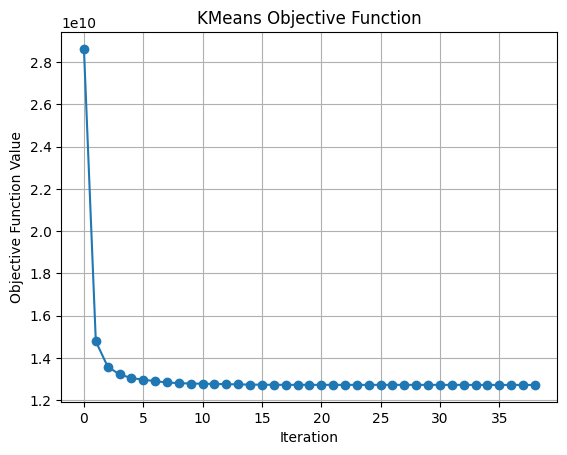
\includegraphics[scale=0.7]{figures/kmeans-objective.png}
	\end{center}

	\pagebreak
	\begin{part}{2} For $K=10$ and for 3 random restarts, print the mean image (aka
		the centroid) for each cluster. There should be 30 total images.
	\end{part}

	\begin{center}
		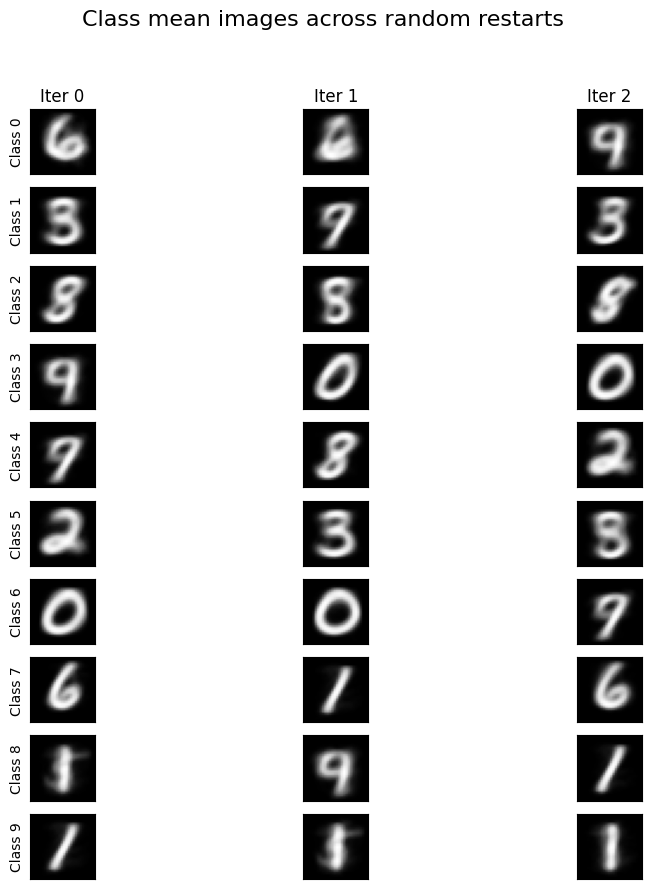
\includegraphics[scale=0.7]{figures/kmeans-class_means.png}
	\end{center}

	\pagebreak
	\begin{part}{3} Repeat Part 2, but before running K-means, standardize or center
		the data such that each pixel has mean 0 and variance 1 (for any
		pixels with zero variance, simply divide by 1). For $K=10$ and 3
		random restarts, show the mean image (centroid) for each
		cluster. Again, present the 30 total images in a single
		plot. Compare to Part 2: How do the centroids visually differ? Why?
	\end{part}

	\begin{center}
		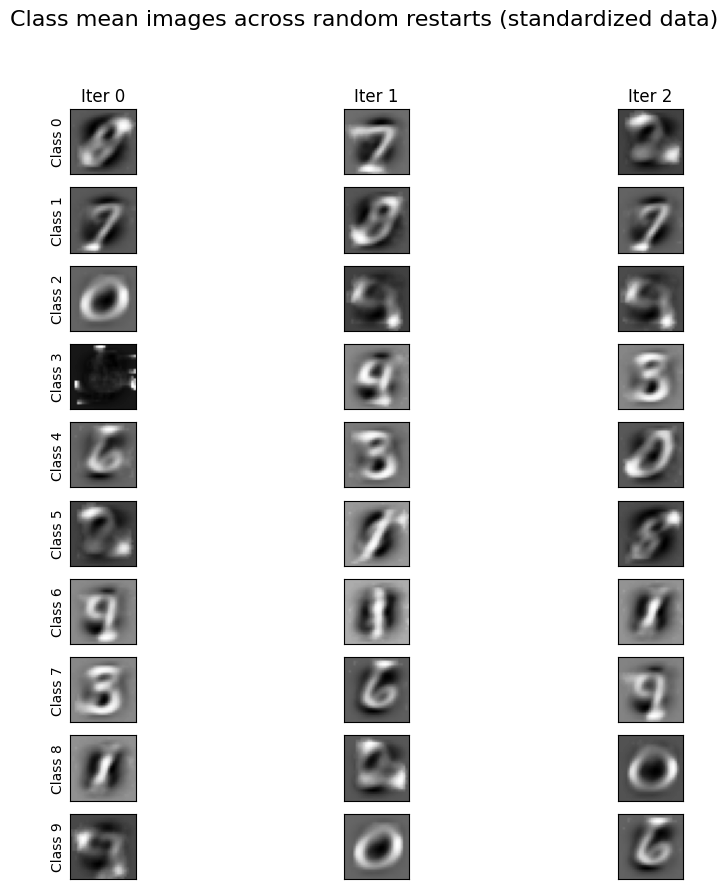
\includegraphics[scale=0.7]{figures/kmeans-class_means_std.png}
	\end{center}

	The centroids for the standardized dataset visually look quite different - there is much lower contrast, the images are lighter and blurrier. This makes sense, since high contrast means higher variance, so if we normalize the variance the constrast would decrease. Similarly, the images are mostly black before standardization so if we normalize the mean they would approach an overall gray shape. Additionally, there are some interesting visual artifacts such as dark spots around in the circle of the zero, although I'm not sure what causes this.

	\pagebreak
	\begin{part}{4} Implement HAC for min, max, and centroid-based linkages. Fit
		these models to the \texttt{small\_dataset}.  For each of these 3
		linkage criteria, find the mean image for each cluster when using $10$ clusters. Display these images (30 total) on a single plot. How do the ``crispness'' of the cluster means and the digits
		represented compare to mean images for k-means?
		Why do we only ask you to run HAC once?
	\end{part}

	\begin{center}
		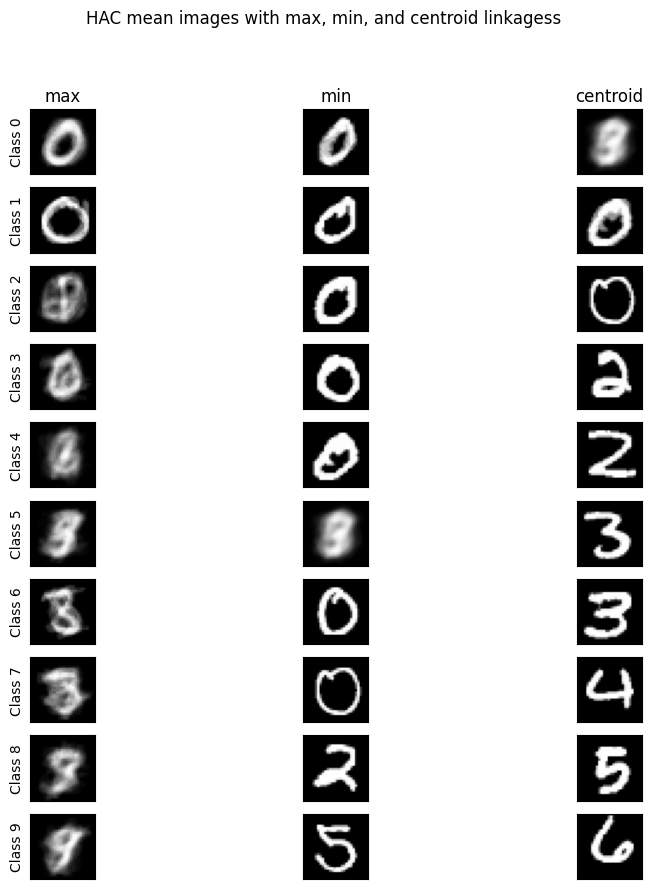
\includegraphics[scale = 0.7]{figures/HAC-class_means.png}
	\end{center}

	The means are less consistently crisp compared to the K-means class means, and this corresponds to cluster sizes. This means that for classes with a lot of elements, the image is not crisp at all, but for classes with not that many elements, the image is very crisp. On the other hand, in K-means, most of the class means are similarly crisp. The reason why we run HAC only once is because it is deterministic so we would get the same results every time.

	\begin{part}{5} For each of the HAC linkages, as well as one of the runs of your
		k-means, make a plot of ``Number of images in cluster" (y-axis)
		v. ``Cluster index" (x-axis) reflecting the assignments during the
		phase of the algorithm when there were $K=10$ clusters. Intuitively, what do these plots tell you about the difference between the clusters produced by the max and min linkage criteria? Going back to the previous part: How does this help explain the crispness and blurriness of some of the clusters?
	\end{part}

	\begin{center}
		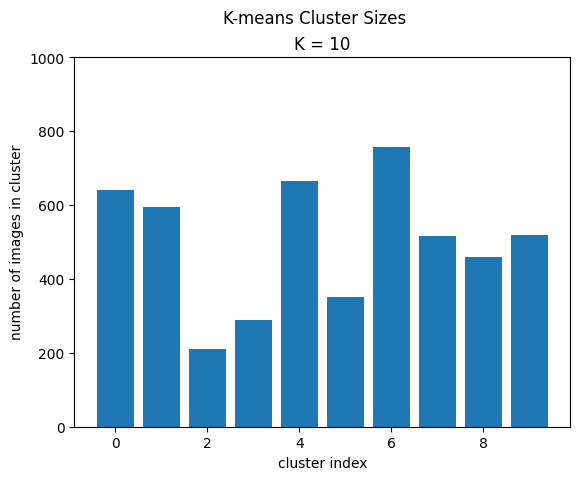
\includegraphics[scale = 0.7]{figures/kmeans-cluster_sizes.png}
		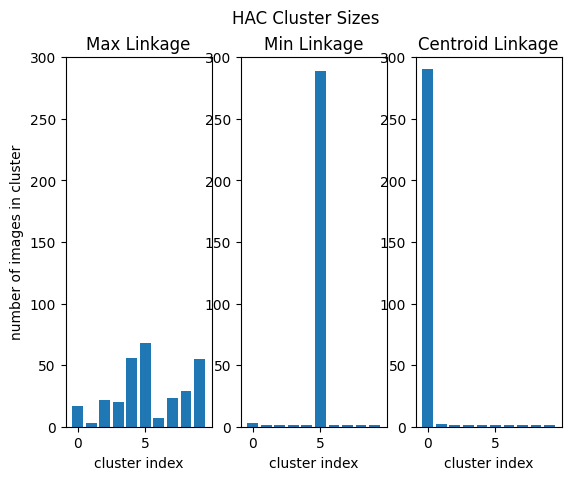
\includegraphics[scale = 0.7]{figures/HAC-cluster_sizes.png}
	\end{center}

	It appears that the max linkage criteria has the most even distribution of clusters, and this corresponds to the increased blurriness in the class means. The min and centroid linkages have a much higher contrast in their cluster sizes, so most of the clusters are crisp while the big clusters are blurry.

	\begin{part}{6} For your K-means with $K = 10$ model and HAC min/max/centroid
		models using $10$ clusters on the \texttt{small\_dataset} images,
		use the \texttt{seaborn} module's \texttt{heatmap} function to plot
		a confusion matrix between each pair of clustering methods.  This
		will produce 6 matrices, one per pair of methods. The cell at the
		$i$th row, $j$th column of your confusion matrix is the number of
		times that an image with the cluster label $j$ of one method has
		cluster $i$ in the second method.  Which HAC is closest to k-means?
		Why might that be?
	\end{part}

	Here is the plot of confusion matrices:
	\begin{center}
		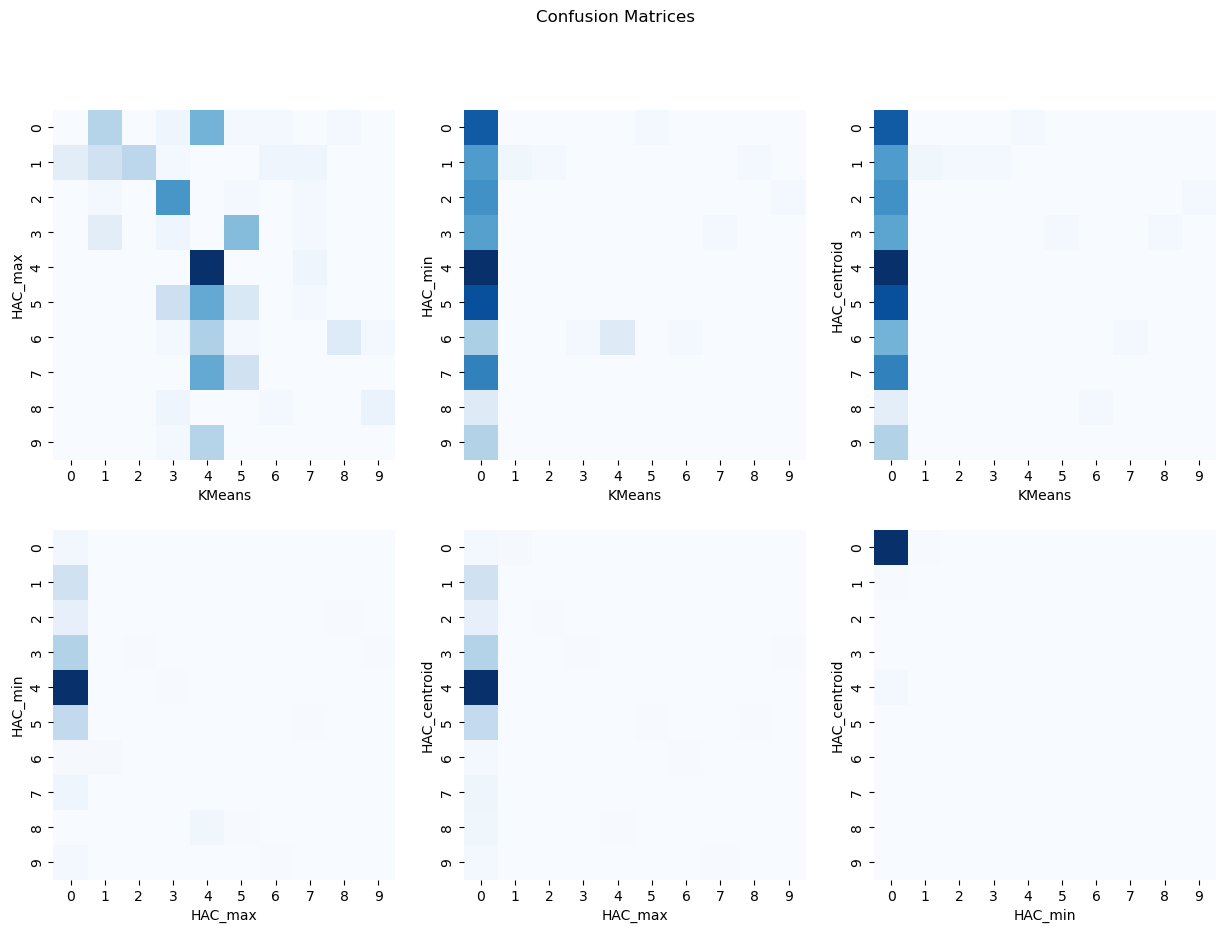
\includegraphics[scale = 0.5]{figures/confusion_matrices.png}
	\end{center}
	It appears that \texttt{HAC\_max} is closest to \texttt{KMeans} which makes sense intuitively since it has the most even spread of cluster sizes, like KMeans. The other \texttt{HAC} cluster runs seem to all center around one massive cluster, which does not resemble any \texttt{KMeans} run which I was able to produce.


	\begin{part}{7} Let's return to the postal service example from HW3.  Do you
		think that clustering is a good way to identify digits, that is,
		first cluster the data, and then, for any new data point, classify
		it based on its cluster?
	\end{part}
	\begin{parts}
		\begin{part}{a} In particular, do you expect the clusters to correspond with the true labels?  Is that a good way to evaluate clustering?
		\end{part}

		The clusters don't appear to correspond to the true labels at all. For example, the digits $3$ and $8$ are clustered together most of the time due to their visual similarity, yet the two versions of the digit $2$ (one with a loop and one without) are usually in separate clusters.

		However, evaluating clustering algorithms based on whether they uncover the true labels may not be the best way to evaluate them. This is more of a reflection of how far the true labels stray from the clustering patterns which the dataset follows.

		\begin{part}{b} In the context of adversaries, how might clusterings be
			attacked?  How is the process similar or different to the process
			for attacking classification models (like kNN and the generative classifiers that we saw in HW2)?
		\end{part}

		One of the main differences between clustering algorithms and kNN/generative classifiers is that clustering are unsupervised. This means that adversarial influences can be more subtle, but affect the distribution of the data in stronger ways. For example, we could inject some brighter regions of pixels into a corner of the image, so that we can achieve our desired clustering outcome. We could also manipulate the clustering algorithm used if we know the distribution of the data, since they all seem to perform quite differently.
	\end{parts}
\end{parts}

\begin{problem}{3}[EthiCS]
Consider the simulation we conducted in class. There you were part of a health-care administration company, Optimizing Health. Optimizing Health is a small startup and you were a developer reporting directly to the CTO. In particular, you were responsible for designing a system that predicts the healthcare needs of an individual. First, you needed to choose a way to predict healthcare needs. You chose between approximating need by:

\begin{itemize}
	\item the predicted healthcare expenditure of that individual
	\item the predicted number of hours an individual is expected to visit the doctor’s office.
	\item the number of diagnoses the patient has received in the past year.
	\item the average prognosis for individuals in that patient’s age and racial groups.
\end{itemize}

As an organization, you settled on predicting healthcare need by predicted healthcare expenditure of that individual given their diagnosis.

Then, you used that predicted healthcare expenditure to assign a "Risk Score" to all patients, and, for patients above a certain cutoffs, you either automatically enrolled them in the a new program you created called the Medical Management Program (high risk) or referred them to their physician (moderate risk).

You discovered that, at a given Risk Score, Black patients are sicker than White patients. The algorithm was therefore less likely to recommend additional care to Black patients who needed it than White patients. 17.7$\%$ of Black patients were being recommended for additional care, while 46.5$\%$ of Black patients required additional care. After these recommendations were used, doctors provided disparate treatment, with Black patients not entering the Medical Management Program as frequently as they require.

All of these (and many unstated but salient) steps can be modeled using causal chains, backward looking responsibility, and forward looking responsibility (as we did in class).

After the terrible outcome, the CEO resigns and you are promoted to lead the organization! This means that any actions you take will be implemented and so you vow to do better.

The first thing you do is decide to rewrite the mission: “Optimizing Health’s new mission is to provide care to individuals who need it but are not currently receiving it, without increasing healthcare disparities across groups.”

\end{problem}

\begin{parts}
	\begin{part}{}
		With this new goal in mind, think through each important choice-point for success and outline (literally draw) a new causal chain (similar to what you did in Scenario Part 4 in class). This time, however, you can recommend choices other than those outlined in the in-class Scenario and above.

		A sufficiently descriptive causal chain will include points that link the mission to, for instance, the choice to use ML, data collection, feature selection, ... , assignment of risk, what to do with risk scores, and so on. Remember to represent actual decision points as ovals and everything else (things that follow directly from decisions) as rectangles. Moreover, flag the decisions that carry moral or ethical responsibility to distinguish them from decisions that do not. At each point in the chain, if that point involves an ethically salient decision, provide your brief rationale for the decision, a brief description of the main argument against it, and your response to that objection. List the individuals who would be morally responsible at each contributing choice point. Finally, briefly describe how the outcome (the last node in your chain) meets the mission objective.
	\end{part}

	\begin{enumerate}
		\item \textbf{Mission Statement}
		      \begin{itemize}
			      \item Decision: Adopting the new mission of providing care to those in need without increasing disparities.
			      \item Ethical Rationale: Ensures equitable healthcare outcomes.
			      \item Main Argument Against: Might increase operational costs significantly.
			      \item Response: The long-term benefits of improved health outcomes and reduced disparities outweigh short-term cost increases.
			      \item Responsibility: CEO and Board of Directors.
		      \end{itemize}

		\item \textbf{Choose to Use Machine Learning (ML)}
		      \begin{itemize}
			      \item Decision: Continue using ML but with revised objectives.
			      \item Ethical Rationale: ML can process complex datasets to identify underserved individuals accurately.
			      \item Main Argument Against: Risk of perpetuating biases.
			      \item Response: Implement bias mitigation strategies in model development.
			      \item Responsibility: CTO, Data Science Team.
		      \end{itemize}

		\item \textbf{Data Collection} - Collect diverse and comprehensive data, ensuring representation of underrepresented groups.

		\item \textbf{Feature Selection}
		      \begin{itemize}
			      \item Decision: Include variables that directly impact health outcomes and variables indicating social determinants of health.
			      \item Ethical Rationale: Acknowledges the broader determinants of health, aiming for more accurate risk assessment.
			      \item Main Argument Against: Privacy concerns and potential misuse of sensitive data.
			      \item Response: Implement strict data governance policies to protect privacy.
			      \item Responsibility: Data Science Team, Data Governance Officer.
		      \end{itemize}

		\item \textbf{Model Development and Training} - Develop and train the model on the selected features, with an emphasis on fairness and equity.

		\item \textbf{Bias Mitigation Strategies}
		      \begin{itemize}
			      \item Decision: Apply techniques to identify and reduce bias in the model.
			      \item Ethical Rationale: Ensures the model does not perpetuate existing healthcare disparities.
			      \item Main Argument Against: May reduce overall accuracy.
			      \item Response: A more equitable model is crucial, even if it slightly compromises on overall accuracy.
			      \item Responsibility: Data Science Team.
		      \end{itemize}

		\item \textbf{Assignment of Risk Scores} - Utilize the ML model to assign risk scores to patients, incorporating bias mitigation outcomes.

		\item \textbf{Action Based on Risk Scores}
		      \begin{itemize}
			      \item Decision: Adjust the threshold for interventions in a way that accounts for the discovered disparities.
			      \item Ethical Rationale: Directs resources to those who are most in need, acknowledging past inequities.
			      \item Main Argument Against: Could be seen as preferential treatment.
			      \item Response: Corrective measures are necessary to address systemic inequities.
			      \item Responsibility: Healthcare Management Team.
		      \end{itemize}

		\item \textbf{Program Enrollment Decisions} - Based on the revised risk scores and thresholds, automatically enroll or refer patients to appropriate programs.

		\item \textbf{Ongoing Evaluation and Adjustment}
		      \begin{itemize}
			      \item Decision: Regularly review and adjust the ML model and its outcomes.
			      \item Ethical Rationale: Ensures the system remains fair and effective over time.
			      \item Main Argument Against: Requires continuous resources.
			      \item Response: Essential for maintaining trust and efficacy in healthcare provision.
			      \item Responsibility: Oversight Committee (includes community representatives).
		      \end{itemize}

		\item \textbf{Outcome: Equitable Healthcare Provision} - Achieving the mission of providing care to those in need without increasing disparities, as evidenced by equitable health outcomes and satisfaction across all patient groups.
	\end{enumerate}
\end{parts}

\end{document}
